\scanpage{20}

\figure{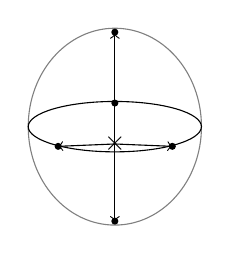
\begin{tikzpicture}[scale=1]
\draw[gray] (0,0) ellipse (1.1 and 1.25);
\draw (0,0) ellipse (1.1 and .32);
\draw[->] (0,-.22)--(0,1.18);
\draw[->] (0,-.22)--(0,-1.2);
\draw[->] (0,-.22)--(-.72,-.25);
\draw[->] (0,-.22)--(.73,-.25);
\node at (0,-.22) {$\times$};
\foreach \p in {(0,1.2),(0,.3),(-.72,-.25),(.73,-.25),(0,-1.2)}{\fill \p circle (.045);}
\end{tikzpicture}}

\figure{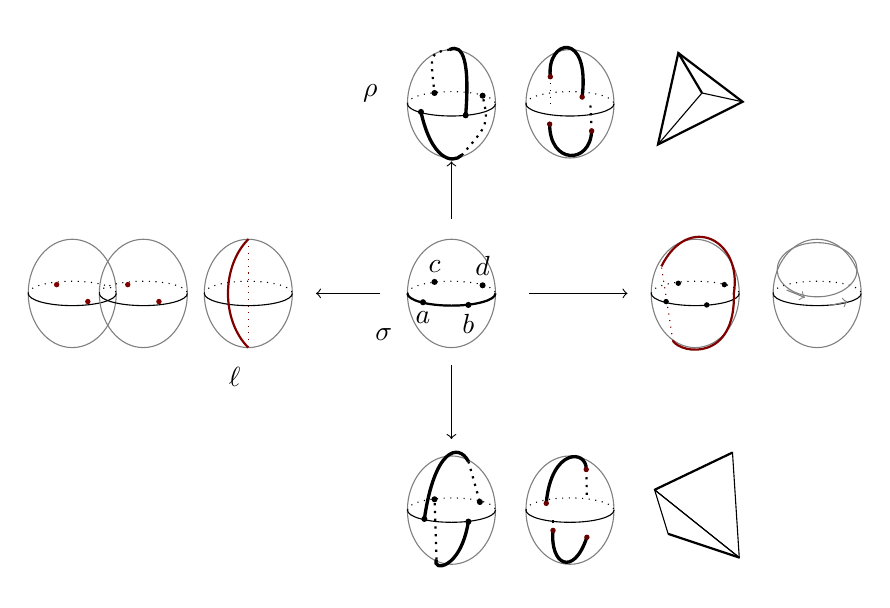
\begin{tikzpicture}[scale=.86]
\foreach \x/\y in {0/0,1.05/0,2.6/0,5.6/0,9.2/0,11/0,5.6/2.8,7.35/2.8,5.6/-3.2,7.35/-3.2}{
\begin{scope}[shift={(\x,\y)}]
\draw[gray] (0,0) ellipse (.65 and .8);
\draw (-.65,0) arc[start angle=180,end angle=360,x radius=.65,y radius=.18];
\draw[dotted] (-.65,0) arc[start angle=180,end angle=0,x radius=.65,y radius=.18];
\end{scope}}
\foreach \x in {0,1.05}{
\fill[red!50!black] (\x-.23,.13) circle (.04);
\fill[red!50!black] (\x+.23,-.12) circle (.04);}
\begin{scope}[shift={(2.6,0)}]
\draw[red!50!black,thick] (0,.8)..controls(-.4,.4)and(-.4,-.4)..(0,-.8);
\draw[red!50!black,dotted] (0,.8)--(0,-.8);
\node[below] at (-.2,-.95) {$\ell$};
\end{scope}
\begin{scope}[shift={(5.6,0)}]
\draw[thick] (-.65,0) arc[start angle=180,end angle=360,x radius=.65,y radius=.18];
\foreach \p in {(-.42,-.13),(.25,-.17),(-.25,.17),(.46,.12)}{\fill \p circle (.045);}
\node[below] at (-.42,-.13) {$a$};
\node[below] at (.25,-.17) {$b$};
\node[above] at (-.25,.17) {$c$};
\node[above] at (.46,.12) {$d$};
\node at (-1,-.6) {$\sigma$};
\end{scope}
\draw[->] (4.55,0)--(3.6,0);
\draw[->] (6.75,0)--(8.2,0);
\draw[->] (5.6,1.1)--(5.6,1.95);
\draw[->] (5.6,-1.05)--(5.6,-2.15);
\begin{scope}[shift={(9.2,0)}]
\draw[red!50!black,thick] (-.5,.4)..controls(-.1,1.2)and(.7,.8)..(.57,0)..controls(.6,-1)and(-.2,-.9)..(-.33,-.7);
\draw[red!50!black,dotted] (-.33,-.7)--(-.5,.4);
\foreach \p in {(-.43,-.12),(.17,-.17),(-.25,.15),(.43,.13)}{\fill \p circle (.04);}
\end{scope}
\begin{scope}[shift={(11,0)}]
\draw[gray] (0,.35) ellipse (.59 and .4);
\draw[->,gray] (-.45,.05)--(-.18,-.06);
\draw[->,gray] (.18,-.18)--(.45,-.12);
\end{scope}
\begin{scope}[shift={(5.6,2.8)}]
\draw[very thick] (-.45,-.12)..controls(-.3,-.8)and(0,-.9)..(.15,-.76);
\draw[dotted,thick] (.15,-.76)..controls(.55,-.3)..(.46,.12);
\draw[very thick] (.21,-.17)..controls(.27,.6)and(.18,.9)..(-.03,.8);
\draw[dotted,thick] (-.03,.8)..controls(-.32,.75)..(-.25,.16);
\foreach \p in {(-.45,-.12),(.21,-.17),(-.25,.16),(.46,.12)}{\fill \p circle (.045);}
\node at (-1.2,.15) {$\rho$};
\end{scope}
\begin{scope}[shift={(7.35,2.8)}]
\draw[very thick] (-.3,-.3)..controls(-.3,-.9)and(.3,-.9)..(.32,-.4);
\draw[dotted,thick] (.32,-.4)--(.3,0);
\draw[very thick] (.18,.1)..controls(.3,1.1)and(-.35,.95)..(-.29,.4);
\draw[dotted] (-.29,.4)--(-.29,0);
\foreach \p in {(-.3,-.3),(.32,-.4),(.18,.1),(-.29,.4)}{\fill[red!40!black] \p circle (.04);}
\end{scope}
\begin{scope}[shift={(9.2,2.8)}]
\draw[thick] (-.55,-.6)--(-.25,.75)--(.7,.03)--cycle;
\draw (-.55,-.6)--(.1,.16)--(.7,.03);
\draw[thick] (-.25,.75)--(.1,.16);
\end{scope}
\begin{scope}[shift={(5.6,-3.2)}]
\draw[very thick] (-.4,-.13)..controls(-.25,.9)and(.1,1)..(.25,.72);
\draw[dotted,thick] (.25,.72)--(.42,.12);
\draw[very thick] (.25,-.17)..controls(.13,-.9)and(-.3,-.9)..(-.22,-.73);
\draw[dotted,thick] (-.22,-.73)--(-.25,.16);
\foreach \p in {(-.4,-.13),(.42,.12),(.25,-.17),(-.25,.16)}{\fill \p circle (.045);}
\end{scope}
\begin{scope}[shift={(7.35,-3.2)}]
\draw[very thick] (-.35,.1)..controls(-.28,.92)and(.25,.9)..(.24,.6);
\draw[dotted,thick] (.24,.6)--(.25,.2);
\draw[very thick] (.25,-.4)..controls(.05,-1)and(-.3,-.8)..(-.25,-.3);
\draw[dotted,thick] (-.25,-.3)--(-.25,-.12);
\foreach \p in {(-.35,.1),(.24,.6),(.25,-.4),(-.25,-.3)}{\fill[red!40!black] \p circle (.04);}
\end{scope}
\begin{scope}[shift={(9.2,-3.2)}]
\draw (-.6,.3)--(.55,.85)--(.65,-.7)--cycle;
\draw[thick] (-.6,.3)--(.55,.85) (-.4,-.35)--(.65,-.7);
\draw (-.6,.3)--(-.4,-.35)--(.65,-.7) (-.6,.3)--(.65,-.7);
\end{scope}
\end{tikzpicture}}

\figure{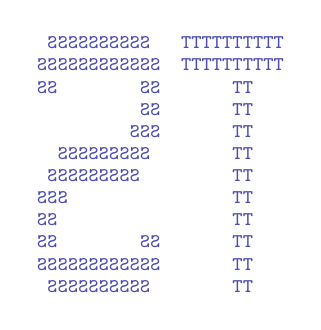
\begin{tikzpicture}
\node[xscale=-1,transform shape,align=left,text=blue!40!gray,font=\ttfamily\scriptsize] {
\unsure{TTTTTTTTTT}\quad\phantom{S}\unsure{SSSSSSSSSS}\phantom{S}\\
\unsure{TTTTTTTTTT}\quad\unsure{SSSSSSSSSSSS}\\
\phantom{TTT}\unsure{TT}\phantom{TTTTT}\quad\unsure{SS}\phantom{SSSSSSSS}\unsure{SS}\\
\phantom{TTT}\unsure{TT}\phantom{TTTTT}\quad\unsure{SS}\phantom{SSSSSSSSSS}\\
\phantom{TTT}\unsure{TT}\phantom{TTTTT}\quad\unsure{SSS}\phantom{SSSSSSSSS}\\
\phantom{TTT}\unsure{TT}\phantom{TTTTT}\quad\phantom{S}\unsure{SSSSSSSSS}\phantom{SS}\\
\phantom{TTT}\unsure{TT}\phantom{TTTTT}\quad\phantom{SS}\unsure{SSSSSSSSS}\phantom{S}\\
\phantom{TTT}\unsure{TT}\phantom{TTTTT}\quad\phantom{SSSSSSSSS}\unsure{SSS}\\
\phantom{TTT}\unsure{TT}\phantom{TTTTT}\quad\phantom{SSSSSSSSSS}\unsure{SS}\\
\phantom{TTT}\unsure{TT}\phantom{TTTTT}\quad\unsure{SS}\phantom{SSSSSSSS}\unsure{SS}\\
\phantom{TTT}\unsure{TT}\phantom{TTTTT}\quad\unsure{SSSSSSSSSSSS}\\
\phantom{TTT}\unsure{TT}\phantom{TTTTT}\quad\phantom{S}\unsure{SSSSSSSSSS}\phantom{S}
};
\end{tikzpicture}}

\[
\begin{aligned}
I&=I_Q=\coprod_{d\in D_Q}d\\
A_Q&=\prod_{d\in D_Q}d\\
C_Q&=\bigwedge_{d\in D_Q}d=\unsure{\perp}\\
\omega_Q&=C_Q\wedge D_Q\\
\omega_I&\simeq\omega_J\simeq C_Q\simeq J\setminus\{Q\}
\end{aligned}
\]

\[
\boxed{\begin{gathered}
a\ b\ c\ d\\
(ad)(bc)=Q_0\\
(b,d)(ac)=Q_1\\
(cd)(ab)=Q_\infty
\end{gathered}}
\]

\[
\underbrace{
(\text{tétraèdre \inserted{orienté}}+\text{diagonale})
\longleftrightarrow
(\text{carré}+\text{codiagonale})
}_{\substack{\omega_I\times J\\ \simeq J\times\omega_I}}
\]

\margin{$\unsure{\omega_I\times J}$}

\figure{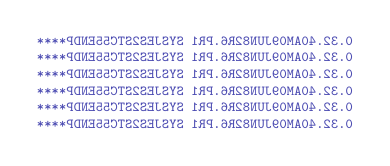
\begin{tikzpicture}
\node[xscale=-1,transform shape,align=left,text=blue!40!gray,font=\ttfamily\tiny] {
\unsure{0.32.40AM09JUN82R6.PR1 SYSJES2STC55ENDP****}\\
\unsure{0.32.40AM09JUN82R6.PR1 SYSJES2STC55ENDP****}\\
\unsure{0.32.40AM09JUN82R6.PR1 SYSJES2STC55ENDP****}\\
\unsure{0.32.40AM09JUN82R6.PR1 SYSJES2STC55ENDP****}\\
\unsure{0.32.40AM09JUN82R6.PR1 SYSJES2STC55ENDP****}\\
\unsure{0.32.40AM09JUN82R6.PR1 SYSJES2STC55ENDP****}
};
\end{tikzpicture}}

\diagram{\begin{tikzcd}
0\arrow[r]&V(J)\arrow[r]&\unsure{\mathfrak S_I}\arrow[r]&\unsure{\mathfrak S_J}\arrow[r]&1
\end{tikzcd}}

\figure{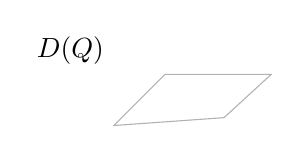
\begin{tikzpicture}[scale=1]
\node[above left] at (0,0.65) {$\unsure{D(Q)}$};
\draw[gray!60] (0,0)--(.65,.65)--(2,.65)--(1.4,.1)--cycle;
\end{tikzpicture}}

\[
\boxed{\left\{\begin{aligned}
\rho^3&=\sigma^2=1\\
\rho\sigma&=\ell
\end{aligned}\right.}
\]

\diagram{\begin{tikzcd}[column sep=small,row sep=large]
1\arrow[r]&
\unsure{\Gamma|\mathcal T}_{0,4}^{!}\arrow[r]\arrow[d,"\simeq",draw=none]&
\unsure{\Gamma|\mathcal T}_{04}^{\deleted{\unsure{!}}}\arrow[r]\arrow[d]&
\unsure{\mathfrak S_4}\arrow[r]\arrow[d]&1\\
1\arrow[r]&
\Pi_{0,3}\arrow[r,very thick]\arrow[d,"\simeq",draw=none]&
\unsure{\Gamma|\mathcal T}_{04}'\arrow[r]&
\unsure{\mathfrak S_3}\arrow[r,dash]&1\\
1\arrow[r]&
\Pi_{0,\unsure{3|5}}^{\unsure{2}}\arrow[r,very thick]&
\unsure{\Gamma|\mathcal T}_{1,1}\arrow[r]\arrow[u]&
\unsure{\widetilde{\mathfrak S}_3}\arrow[u]
\end{tikzcd}}

\margin{cart}

\[
\begin{aligned}
\unsure{\mathfrak S_4}&\simeq\operatorname{Aff}(2,\mathbb Z/2\mathbb Z)\\
\unsure{\mathfrak S_3}&\quad\text{``}\operatorname{Sl}(2,\mathbb Z/2\mathbb Z)\\
\unsure{\widetilde{\mathfrak S}_3}&\simeq\operatorname{Sl}(2,\mathbb Z/4\mathbb Z)/-\\
\unsure{\Gamma|\mathcal T}_{1,1}&\simeq\operatorname{Sl}(2,\mathbb Z)
\end{aligned}
\]

\margin{19}
